% HyPSO-QCO, DAC 2027 submission -- revised version.
% Build (from paper/final):  pdflatex hypso_qco_dac27_revised && pdflatex hypso_qco_dac27_revised
% Figures: ../figures_rev (generated by paper/rev_figs.py), fig2_overview.pdf (unchanged from the
% submission), Table I: ../tables_rev.tex (generated by qcpso.bench.report_revision --latex).
\documentclass[conference,letterpaper]{IEEEtran}
\usepackage[T1]{fontenc}
\usepackage{amsmath,amssymb,amsfonts}
\usepackage{bm}
\usepackage{graphicx}
\usepackage{booktabs}
\usepackage{cite}
\usepackage{url}
\usepackage[hidelinks]{hyperref}
\graphicspath{{../figures_rev/}{./}}

\newcommand{\cir}[1]{\texttt{#1}}
\newcommand{\tool}[1]{\texttt{#1}}
\newcommand{\hypso}{HyPSO-QCO}
\newtheorem{proposition}{Proposition}
\newtheorem{definition}{Definition}
\newcommand{\U}{\mathrm{U3}}

\begin{document}

\title{HyPSO-QCO: Connectivity-Preserving Resynthesis\\ and Exact Swarm Search for Hardware-Mapped\\ Quantum Circuits}

\author{\IEEEauthorblockN{Anonymous Author(s)}
\IEEEauthorblockA{Paper under double-blind review}}

\maketitle

\begin{abstract}
Two-qubit gates dominate the error budget of superconducting quantum processors, yet circuits that a
production transpiler has already mapped and optimised leave little room for improvement: the result must
keep the physical qubits, coupled pairs and native gate directions of its input. We present \hypso{}, which
re-optimises such circuits with two layers of exact search. A particle swarm searches the decisions of a
semantics-preserving compiler, so every candidate is equivalent to the input by construction; a memetic phase
then deletes CNOT gates only inside each block's own CNOT skeleton, so no new qubit interaction can appear,
with an end-to-end error bounded by checked block residuals. On ten circuits transpiled by Qiskit at
optimisation level~3 for a 127-qubit IBM Eagle device (1,898 to 357,535 gates), \hypso{}, in a configuration
fixed before the runs, used the fewest two-qubit (ECR) gates of all evaluated tools on every circuit within
15 minutes. Over three seeds, it removed 33.4\% of the ECR gates on average, against 21.5\% for GUOQ with a
four times longer budget, 8.9\% for BQSKit's deletion-only workflow, 4.1\% for TKET and 0.1\% for QUESO
(one-sided Wilcoxon $p = 0.001$ against each). Its worst seed beat GUOQ's best run on each of the seven
smaller circuits, it passed GUOQ's 60-minute result after a median of 1.2 minutes, and every checked output
was numerically exact.
\end{abstract}

\section{Introduction}



Quantum programs must be compiled to the native gates and qubit connectivity of a device. On IBM's 127-qubit
Eagle processors, the native gate set is $\{rz, sx, x, ecr\}$; $rz$ is a virtual frame change~\cite{mckay2017},
so the physical cost lies in the $sx$ and $x$ gates and, above all, in the two-qubit echoed cross-resonance
(ECR) gates, each more than an order of magnitude more error-prone than a physical single-qubit gate. The ECR
count is therefore the primary objective.

\begin{figure}[t]
\centering
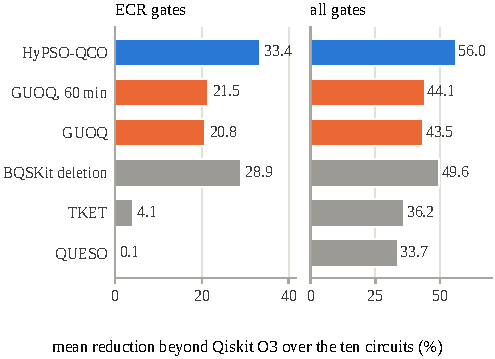
\includegraphics{rev_fig1_mean_reduction.pdf}
\caption{Mean reduction beyond Qiskit O3 over the ten IBM Eagle benchmarks (15\,min per circuit for the
anytime tools; GUOQ also 60\,min; \hypso{} and GUOQ: mean of three seeds on the seven smaller circuits; IBM AI
synthesis: the eight circuits it finished). \hypso{} used the fewest ECR gates on all ten circuits (one-sided
Wilcoxon $p = 0.001$ against each tool that ran on all ten).}
\label{fig:mean}
\end{figure}

A circuit is often available only after a production transpiler, such as Qiskit at optimisation level~3
(Qiskit O3)~\cite{qiskit}, has laid it out, routed it and optimised it. Re-optimising it is tightly
constrained: the result must stay on the same physical qubits, may couple only pairs that the input already
couples, must apply every ECR gate in its native direction, and must improve on a circuit that a level-3
optimiser has already simplified. Mapping-preserving rewriters find little to remove: QUESO~\cite{queso}
removed at most 0.6\% of the ECR gates of any of our circuits, and TKET's connectivity-preserving
passes~\cite{tket} at most 0.8\% on five of ten. ZX-calculus simplification~\cite{duncan2020,pyzx},
VOQC~\cite{voqc} and TKET's full peephole optimisation can couple uncoupled qubits. Numerical
resynthesis~\cite{qsearch,qfast,leap}, applied block-wise by BQSKit~\cite{bqskit} and interleaved with
rewriting by GUOQ~\cite{guoq}, reaches further but meets two obstacles: synthesis may create new interactions
(GUOQ needed a small patch to return valid circuits under our contract), and it must scale: on our two
largest benchmarks (93,235 and 357,535 gates), GUOQ removed at most 0.4\% of the ECR gates in 15 minutes and
0.7\% in 60 minutes, and BQSKit's deletion-only workflow at most 0.9\% of the remaining CNOTs.

\begin{figure*}[t]
\centering
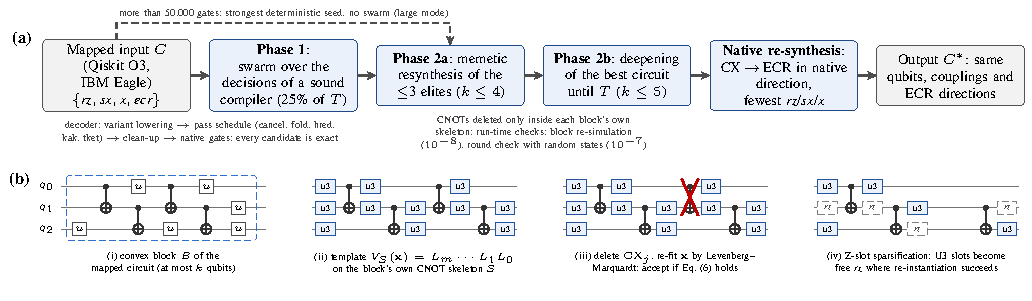
\includegraphics[width=\textwidth]{fig2_overview.pdf}
\caption{\hypso{} at a glance. (a) Phase~1 searches the decisions of a sound compiler, so every candidate
is equivalent to the input; phase~2 refines up to three elites by connectivity-preserving memetic
resynthesis until they stall (2a) and deepens the best circuit with larger blocks until the deadline (2b).
On mapped circuits, we run resynthesis only: phase~2 starts from the strongest deterministic seed and
receives the whole budget. (b)~One resynthesis step on an illustrative block: only CNOTs of the block's own
skeleton can disappear, so the device mapping is unchanged.}
\label{fig:overview}
\end{figure*}

We present \hypso{}, which re-optimises mapped circuits under this strict contract with two layers of exact
search (Fig.~\ref{fig:overview}). In phase~1, the particles of a swarm encode the free decisions of a
semantics-preserving compiler (which exact decomposition each multi-variant gate uses and which sound passes
run), so every candidate is equivalent to the input by construction. In phase~2, a memetic local search
resynthesises blocks of the best candidates by deleting CNOT gates only inside each block's own CNOT
skeleton, so no new qubit interaction can appear. Our contributions are as follows.
\begin{itemize}
\item \textbf{Connectivity-preserving memetic resynthesis} (Section~\ref{sec:phase2}). An exact start,
Schmidt-rank pruning, warm-started Levenberg--Marquardt fits, Z-slot sparsification into free virtual $rz$
gates and adaptive selection among 12 strategies make CNOT deletion effective on circuits already optimised
by Qiskit O3; the end-to-end error is bounded by the checked block residuals
(Proposition~\ref{prop:sound}).
\item \textbf{Exact decision-space search} (Section~\ref{sec:phase1}). A categorical swarm searches compiler
decisions over all 108 minimal 6-CNOT and 12 nearest-neighbour 8-CNOT Toffoli networks and 16 exact
lowerings per ECR gate; on logical circuits, it significantly outperforms canonical PSO.
\item \textbf{Evaluation against the strongest baselines under one contract} (Section~\ref{sec:results}).
\hypso{} used the fewest ECR gates of TKET, QUESO, BQSKit's deletion-only workflow, IBM's AI synthesis
passes and GUOQ on every circuit (Fig.~\ref{fig:mean}), over three seeds and against GUOQ with four times its
budget: it removed 33.4\% of the ECR gates on average, against 21.5\% for GUOQ in 60 minutes and 8.9\% for
BQSKit, with numerically exact outputs.
\end{itemize}

\section{Background and Related Work}

\subsection{Native Gates, Equivalence and CNOT Lower Bounds}
On IBM Eagle devices, $rz(\theta)$ is virtual, $sx$ and $x$ are physical, and every single-qubit unitary
equals $rz\,sx\,rz\,sx\,rz$ up to a phase~\cite{nielsen}, i.e., at most two physical gates. An $ecr$ gate
acts only on coupled pairs, in one native direction, and equals a CNOT up to single-qubit Clifford gates, so
a CNOT in either orientation on a coupled pair costs one $ecr$ gate. Circuits $C$ and $C'$ on the same
qubits are equivalent if $U(C') = e^{i\varphi}U(C)$ for some $\varphi\in\mathbb{R}$. Two-qubit blocks need
at most three CNOTs, with the minimum computable analytically~\cite{shende2004}; for larger blocks, the
operator Schmidt rank gives a lower bound, since a gate on one side of a cut has rank one and a CNOT across
it rank two, so $m$ CNOTs across a cut implement only operators of rank at most $2^m$.

\subsection{Related Work}
\textbf{Rewriting and compilers.} Rule-based optimisers apply exact local
rewrites~\cite{voqc,nam2018,iten2022}, and production compilers~\cite{qiskit,tket} add layout and
routing~\cite{sabre}; \hypso{}'s decoder reuses the cancellation, rotation merging and Hadamard reduction of
Nam et al.~\cite{nam2018}. Superoptimisers such as Quartz~\cite{quartz} and QUESO~\cite{queso} generate
verified rewrite rules, and Quarl~\cite{quarl} learns which rule to apply but needs a trained GPU model.

\textbf{Numerical resynthesis.} QSearch~\cite{qsearch}, QFAST~\cite{qfast} and LEAP~\cite{leap}
instantiate parameterised templates. BQSKit~\cite{bqskit} resynthesises the blocks of a partitioned circuit
and deletes gates while re-instantiation succeeds, QFactor~\cite{qfactor} scales this deletion beyond 100
qubits, and GUOQ~\cite{guoq} interleaves resynthesis with fast rewriting; reinforcement-learning synthesis
re-synthesises Clifford and Pauli-network blocks after routing~\cite{kremer2024,dubal2025}. \hypso{} builds
on deletion by re-instantiation and adds an exact start, Schmidt-rank pruning, sparsification to virtual $rz$
gates and adaptive scheduling over the elites of an exact search; we compare against BQSKit's deletion-only
workflow under the same budget and cores.

\textbf{Search over compiler decisions.} Per-program pass selection is classical
autotuning~\cite{cooper1999,opentuner} and has been learned for quantum compilers~\cite{quetschlich2023}.
Swarm and evolutionary circuit synthesis~\cite{datta2013,zelinka2023,hidayat2025} encodes gates directly in
the particle, so most candidates are not equivalent to the target; \hypso{}'s particles encode decisions of a
sound compiler, with a categorical update after Strasser et al.~\cite{strasser2016}.

\section{Problem Formulation}
Let $D = (V, A)$ be the directed coupling graph of the device, where $(q, q')\in A$ means that $ecr$ can act
on $q$ and $q'$ in this order, and let $\mathcal{G} = \{rz, sx, x, ecr\}$. A circuit $C$ over $\mathcal{G}$
acts on the physical qubits $Q(C)\subseteq V$, and its interaction set $I(C) = \{\{q, q'\} : C$ has a
two-qubit gate on $q$ and $q'\}$ records the pairs that it couples. In the mapped input, every $ecr$ gate
acts on a pair in $A$ in its native direction.

\begin{definition}[Re-optimisation contract]
$C'$ is an admissible output for the mapped input $C$ if (i)~$C'$ acts on the physical qubits of $C$ and
$U(C') = e^{i\varphi}U(C)$ for some $\varphi\in\mathbb{R}$, with neither a relabelling of the qubits nor a
final permutation; (ii)~$I(C')\subseteq I(C)$, and every $ecr$ gate of $C'$ acts on a pair in $A$ in the
native direction; and (iii)~every gate of $C'$ belongs to $\mathcal{G}$.
\end{definition}

Condition (ii) is stricter than respecting the device: the output needs neither new routing nor new
calibrated pairs. The same contract applies to every evaluated optimiser. Within a wall-clock budget $T$ per
circuit, \hypso{} minimises, in lexicographic order,
\begin{equation}
f(C') = \bigl(n_{ecr}(C'),\, n_{tot}(C'),\, d(C')\bigr),
\end{equation}
the numbers of $ecr$ gates and of all gates and the depth. Because $rz$ is virtual, we also report the
physical single-qubit gates $n_{1q} = n_{sx} + n_{x}$ and the estimated success probability
\begin{equation}
P(C') = (1-\varepsilon_{ecr})^{n_{ecr}(C')}\,(1-\varepsilon_{1q})^{n_{1q}(C')},
\end{equation}
with $\varepsilon_{ecr} = 7\times10^{-3}$ and $\varepsilon_{1q} = 2.5\times10^{-4}$, a model estimate rather
than a measurement on hardware. Every metric $m$ is reported as the reduction $1 - m(C')/m(C)$.

\section{The HyPSO-QCO Framework}

\subsection{Overview}
Phase~1 runs the swarm for 25\% of the budget $T$ (Fig.~\ref{fig:overview}(a)). Phase~2a refines up to three
distinct elites by memetic resynthesis with blocks of up to four qubits, each until it stalls, and phase~2b
deepens the best circuit with blocks of up to five qubits until the deadline; a final native re-synthesis
returns the circuit to $\mathcal{G}$. Above 50,000 gates, one decode takes minutes, so \hypso{} skips the
swarm and starts phase~2 from the strongest deterministic seed (large mode). On mapped circuits, the swarm
does not pay for itself at short budgets (Section~\ref{sec:rq4}), so we use this resynthesis-only procedure
for all of them.

\subsection{Phase 1: Exact Decision-Space Search}\label{sec:phase1}
\textbf{Decoder.} A particle is a vector of genes in $[0, 1)$ that a semantics-preserving decoder interprets.
It lowers every multi-variant gate with the variant that its gene selects (for Toffoli and CCZ gates, one of
all 108 minimal 6-CNOT or 12 nearest-neighbour 8-CNOT networks, times T/T$^\dagger$ polarity and placement;
orientations of CZ, SWAP, CP, CRZ, RZZ/RXX/RZX and CSWAP; for each ECR gate, one of 16 exact Clifford
lowerings to a CNOT) and runs six pass slots, each one of \{skip, cancel, fold, hred, fold+cancel, kak\}:
commutation-aware cancellation, path-sum phase folding, Hadamard reduction~\cite{nam2018} and optimal
two-qubit resynthesis~\cite{shende2004}. In IBM mode, a slot may also run TKET's \tool{KAKDecomposition} and
\tool{CliffordSimp} without swaps (tket), accepted only if a simulation confirms equivalence to $10^{-9}$. A
clean-up fix point and a native re-synthesis follow: each CNOT becomes one $ecr$ gate in its native
direction with the best of 64 exact Clifford wrappings, and each single-qubit run takes the fewest gates over
$\{rz, sx, x\}$. Genes are keyed by provenance tags that every emitted gate carries, so a gene means the same
decision in every particle.

\textbf{Swarm dynamics.} The decisions are nominal, so the arithmetic of canonical
PSO~\cite{kennedy1995,clerc2002} is meaningless for them. Following Strasser et al.~\cite{strasser2016},
particle $i$ holds a probability vector $\bm{\pi}_{ij}$ over the options of each nominal gene $j$ and a
velocity $\mathbf{w}_{ij}$:
\begin{align}
\mathbf{w}_{ij} &\leftarrow \chi\bigl[\mathbf{w}_{ij} + c_1 r_1\bigl(e(p_{ij}) - \bm{\pi}_{ij}\bigr)
 + c_2 r_2\bigl(e(l_{ij}) - \bm{\pi}_{ij}\bigr)\bigr],\\
\bm{\pi}_{ij} &\leftarrow \mathrm{normalise}\bigl(\max(\bm{\pi}_{ij} + \mathbf{w}_{ij}, 0)\bigr),
\end{align}
where $e(\cdot)$ is the one-hot encoding, $p_{ij}$ and $l_{ij}$ are the options of gene $j$ in the personal
and neighbourhood bests, and $r_1, r_2$ are uniform in $[0, 1)$; genes are sampled from $\bm{\pi}_{ij}$ with
an exploration floor of 0.02 ($\chi = 0.7298$, $c_1 = c_2 = 1.49618$, 16 particles). Continuous genes, such
as the layout and SABRE~\cite{sabre} parameters of logical circuits, use standard or quantum-behaved
PSO~\cite{sun2004}. The swarm switches from a von Neumann topology to gbest halfway~\cite{kennedy2002}, uses
opposition-based initialisation~\cite{tizhoosh2005}, partial restarts and a probability-matching local
search~\cite{thierens2005}, and is seeded with three elites of the deterministic compiler, so it is never
worse than greedy compilation.

\subsection{Phase 2: Connectivity-Preserving Memetic Resynthesis}\label{sec:phase2}
Phase~2 works on a $\{1q, \mathrm{CX}\}$ representation of the circuit and proceeds in rounds
(Fig.~\ref{fig:overview}(b)).

\textbf{Partitioning.} A round cuts the circuit into convex blocks of at most $k$ qubits ($k = 3$, 4 or 5)
with a greedy scan and reinserts them by contracting the circuit's directed acyclic graph and re-linearising
it topologically.

\textbf{Template and exact start.} For a block $B$ with unitary $U$ and CNOT skeleton
$S = (\mathrm{CX}_1, \ldots, \mathrm{CX}_m)$, the template is
\begin{equation}
V_S(\mathbf{x}) = L_m\cdots L_1 L_0,\qquad L_j = (\U\otimes\U)\,\mathrm{CX}_j,
\end{equation}
where $L_0$ is a layer of U3 gates on the block's qubits and $\mathbf{x}$ collects their parameters. Every
two-qubit gate of $V_S$ is a CNOT of the block's own skeleton, so deleting CNOTs can never create a new qubit
interaction. The exact start folds every single-qubit run into the U3 slot after the preceding CNOT on its
qubit, so $V_S(\mathbf{x}_0) = U$ before any deletion.

\textbf{CNOT deletion.} The operator tries the CNOTs one by one, in a backward and then a forward sweep.
After each tentative deletion, it re-instantiates the shorter template by Levenberg--Marquardt
optimisation~\cite{nocedal} with an analytic, vectorised Jacobian, warm-started from the previous solution
and aborted early on stagnation; successful fits need a median of about 11 iterations. A deletion is
accepted if
\begin{equation}\label{eq:accept}
\min_{\varphi}\bigl\|V_{S\setminus \mathrm{CX}_j}(\mathbf{x}) - e^{i\varphi}U\bigr\|_F < 10^{-10}.
\end{equation}
Deletions that cannot succeed are skipped: across a cut that separates one qubit from the rest of the block,
a template with too few CNOTs across the cut cannot reach the operator Schmidt rank of $U$. Three-qubit
blocks with more than 20 CNOTs are first refitted to a generic alternating 20-CNOT template on the block's
own two coupled pairs, and a deep strategy adds two PSO-seeded restarts per deletion and deletes CNOT pairs
on the same qubit pair.

\textbf{Z-slot sparsification.} After the deletions, each U3 slot of the block is tentatively restricted to
an $rz$ rotation, which is free on IBM hardware, and the block is re-instantiated; slots for which
Eq.~\eqref{eq:accept} still holds stay $rz$.

\textbf{Schedule.} Probability matching~\cite{thierens2005} rewards CNOTs saved per second and chooses among
12 strategies, which combine the scan direction, random cuts, the block size and restarts. Blocks run
largest-first in a pool of four worker processes, results are memoised, and a round is accepted only if the
CNOT count did not increase. Phase~2a refines each elite until every strategy has failed twice in a row;
phase~2b continues on the best circuit until the deadline.

\subsection{Soundness}
\begin{proposition}[Soundness]\label{prop:sound}
Let $C'$ be the output of \hypso{} for the mapped input $C$. (a)~Every phase-1 candidate $C_x$ satisfies
$U(C_x) = e^{i\varphi}U(C)$, exactly up to rounding for the built-in steps and within the checked $10^{-9}$
for the tket step. (b)~$I(C')\subseteq I(C)$, and every $ecr$ gate of $C'$ acts in the native direction of
its pair. (c)~If every step $j$ that is not exact up to rounding, i.e., every accepted block replacement and
tket step, deviates from the subcircuit that it replaces by at most $\varepsilon_j$ in spectral norm, up to a
phase, then $\min_\varphi\|U(C') - e^{i\varphi}U(C)\|_2 \le \sum_j \varepsilon_j$.
\end{proposition}

\emph{Proof sketch:} (a)~Each variant is an exact decomposition, each built-in pass is a sound
rewrite~\cite{shende2004,nam2018}, the tket step is accepted only after its check, and equivalence up to a
phase is preserved under composition. (b)~Deletion only removes elements of $S$; the refit and the clean-up
use only the block's own pairs; Z-slot sparsification changes single-qubit slots; contraction and
re-linearisation add no gate; and native re-synthesis maps each CNOT on $\{q, q'\}$ to one $ecr$ gate on the
same pair in its native direction. (c)~For unitaries,
$V_m\cdots V_1 - U_m\cdots U_1 = \sum_j V_m\cdots V_{j+1}(V_j - U_j)U_{j-1}\cdots U_1$, so spectral-norm
errors add; embedding a block into the full circuit preserves its spectral norm, and the blocks' phases
combine into one global phase.\hfill$\blacksquare$

Part~(b) makes condition~(ii) of Definition~1 structural. Part~(c) turns block-wise checks into an
end-to-end guarantee: as the Frobenius norm bounds the spectral norm, Eq.~\eqref{eq:accept} gives
$\varepsilon_j < 10^{-10}$ for every fitted block, so $N$ accepted replacements contribute less than
$N\cdot10^{-10}$, even where whole-circuit simulation is infeasible. In our runs, $N$ ranged from 39 to 1,209,
the re-simulated block errors summed to at most $2.2\times10^{-8}$ per output, and the 111 and 465 TKET blocks
of the large-mode seeds added at most $9.2\times10^{-11}$. At run time, every replaced block is also
re-simulated (tolerance $10^{-8}$) and, for up to 20 used qubits, every accepted round is checked with random
states ($10^{-7}$). TKET's \tool{SynthesiseTket} is excluded because it dropped an $rz(3.8\times10^{-4})$
rotation.

\section{Experimental Setup}\label{sec:setup}

% Generated by `python -m qcpso.bench.report_revision --latex paper/tables_rev.tex` -- do not edit.
% Requires \usepackage{booktabs}.

\begin{table*}[t]\centering\scriptsize\setlength{\tabcolsep}{2.3pt}
\caption{ECR / total native gate count after re-optimisation (15\,min per circuit for the anytime tools, GUOQ also 60\,min; mean\,$\pm$\,sd of the ECR count over three seeds on the seven smaller circuits, one seed on the large ones; fewest ECR gates and fewest total gates in bold). The input is Qiskit~O3's transpilation for a 127-qubit IBM Eagle device; $q$: used qubits. Margin: ECR reduction of HyPSO-QCO relative to the best other result on the circuit at any budget. HyPSO-QCO won on all ten circuits against each tool in ECR gates (one-sided Wilcoxon $p = 0.001$).}
\label{tab:main}
\begin{tabular}{l r r rrrrrrrr r}\toprule
circuit & $q$ & input (Qiskit O3) & TKET & QUESO & BQSKit del. & IBM AI & GUOQ 15\,min & GUOQ 60\,min & TKET$\to$GUOQ & HyPSO-QCO & margin \\\midrule
mult\_8 & 8 & 311\,/\,1{,}898 & 299\,/\,1{,}402 & 311\,/\,1{,}337 & 221\,/\,956 & 308\,/\,1{,}473 & 200$\pm$8\,/\,1{,}210 & 191\,/\,1{,}192 & -- & \textbf{155$\pm$2}\,/\,\textbf{796} & 18.8\% \\
heisenberg\_8 & 8 & 420\,/\,2{,}127 & 420\,/\,1{,}455 & 420\,/\,\textbf{1{,}217} & 399\,/\,1{,}270 & 420\,/\,1{,}469 & 326$\pm$9\,/\,1{,}606 & 322\,/\,1{,}652 & -- & \textbf{265$\pm$8}\,/\,1{,}229 & 17.7\% \\
add\_17 & 17 & 499\,/\,2{,}812 & 495\,/\,2{,}203 & 499\,/\,2{,}108 & 470\,/\,1{,}891 & 495\,/\,2{,}182 & 415$\pm$4\,/\,1{,}987 & 414\,/\,1{,}907 & -- & \textbf{391$\pm$2}\,/\,\textbf{1{,}676} & 5.5\% \\
qae\_17 & 17 & 541\,/\,3{,}033 & 537\,/\,2{,}368 & 541\,/\,2{,}301 & 501\,/\,2{,}063 & 541\,/\,2{,}409 & 430$\pm$7\,/\,2{,}093 & 436\,/\,2{,}143 & -- & \textbf{416$\pm$1}\,/\,\textbf{1{,}785} & 3.3\% \\
qft\_16 & 16 & 614\,/\,3{,}444 & 610\,/\,2{,}651 & 614\,/\,2{,}691 & 583\,/\,2{,}253 & 612\,/\,2{,}666 & 532$\pm$4\,/\,2{,}494 & 529\,/\,2{,}447 & -- & \textbf{514$\pm$7}\,/\,\textbf{2{,}149} & 2.9\% \\
hubbard\_8 & 8 & 1{,}344\,/\,8{,}125 & 1{,}251\,/\,5{,}174 & 1{,}336\,/\,6{,}204 & 1{,}243\,/\,5{,}057 & 1{,}221\,/\,5{,}192 & 1{,}138$\pm$8\,/\,4{,}760 & 1{,}130\,/\,4{,}654 & -- & \textbf{852$\pm$38}\,/\,\textbf{3{,}336} & 24.6\% \\
hhl\_8 & 8 & 2{,}377\,/\,18{,}165 & 2{,}365\,/\,14{,}780 & 2{,}377\,/\,16{,}069 & 2{,}150\,/\,13{,}316 & -- & 475$\pm$16\,/\,2{,}805 & 468\,/\,2{,}742 & -- & \textbf{291$\pm$8}\,/\,\textbf{1{,}618} & 37.7\% \\
heisenberg\_32 & 32 & 3{,}942\,/\,58{,}848 & 3{,}834\,/\,14{,}100 & 3{,}942\,/\,14{,}544 & 3{,}808\,/\,14{,}495 & -- & 3{,}805\,/\,14{,}438 & 3{,}719\,/\,13{,}923 & 3{,}741\,/\,14{,}175 & \textbf{3{,}325}\,/\,\textbf{12{,}678} & 10.6\% \\
grover\_10 & 10 & 16{,}397\,/\,93{,}235 & 14{,}453\,/\,57{,}497 & 16{,}397\,/\,74{,}687 & 15{,}860\,/\,56{,}549 & -- & 16{,}392\,/\,72{,}828 & 16{,}380\,/\,71{,}699 & 14{,}445\,/\,56{,}972 & \textbf{12{,}163}\,/\,\textbf{54{,}671} & 15.8\% \\
hubbard\_18 & 31 & 33{,}958\,/\,357{,}535 & 29{,}547\,/\,112{,}902 & 33{,}926\,/\,131{,}273 & 29{,}690\,/\,129{,}229 & -- & 33{,}829\,/\,131{,}019 & 33{,}727\,/\,130{,}582 & 29{,}543\,/\,112{,}898 & \textbf{27{,}224}\,/\,\textbf{104{,}737} & 7.8\% \\
\midrule
mean reduction & & -- & 4.1\%\,/\,36.2\% & 0.1\%\,/\,33.7\% & 8.9\%\,/\,43.2\% & 1.9\%\,/\,25.8\% (6) & 20.8\%\,/\,43.5\% & 21.5\%\,/\,44.1\% & 10.0\%\,/\,61.1\% (3) & 33.4\%\,/\,56.0\% & 14.5\% \\
\bottomrule\end{tabular}\end{table*}


\textbf{Benchmarks.} Table~\ref{tab:main} lists the ten circuits: 8 to 32 used qubits and 1,898 to 357,535
gates, all transpiled by Qiskit O3 for a 127-qubit IBM Eagle coupling map, so every reduction comes on top of
Qiskit O3. None appears in the related tools' published suites, so every tool was run here.

\textbf{Tools.} TKET~\cite{tket} (pytket 2.18.4) ran to a fixed point of \tool{SynthesiseTket},
\tool{KAKDecomposition} and \tool{CliffordSimp}, the latter two without swaps (\tool{FullPeepholeOptimise}
can couple uncoupled qubits). QUESO~\cite{queso} and GUOQ~\cite{guoq} ran from the GUOQ binary (commit
8c4c3a5) with their authors' flags and \tool{-preserve-mapping}; GUOQ used \tool{-opt TWO\_Q} with BQSKit
1.2.1 resynthesis and a small patch that makes its resynthesis connectivity-aware, without which it cannot
return a valid circuit under our contract; the patch only restricts GUOQ. On the large circuits, GUOQ also
ran on TKET's output for the rest of the 15 minutes (TKET$\to$GUOQ). BQSKit~\cite{bqskit} ran its
deletion-only workflow (partitioning, \tool{ScanningGateRemovalPass} per block, unfolding) on four workers
for 15 minutes, growing the blocks from three to five qubits whenever a sweep stops improving, so that the
whole budget is used. Its threshold bounds a block's Hilbert--Schmidt cost, which grows with the square of
the operator error: at the default $10^{-8}$, its \cir{heisenberg\_8} output was $1.4\times10^{-4}$ off, so we
used $10^{-15}$ (399 instead of 402 ECR gates there) and level-1 instantiation, which beat level~2 in a pilot
(\cir{mult\_8}: 221 against 246). It received the circuit after \hypso{}'s exact final stage (two-qubit
resynthesis, cancellation, U3 fusion), which alone removes 0--12\% of the CNOTs and can only favour it. IBM's
AI synthesis passes~\cite{kremer2024,dubal2025} (qiskit-ibm-transpiler 0.18, local models) re-synthesised
Clifford, linear-function and permutation blocks on the input's coupled pairs; their Pauli-network synthesis
returned non-equivalent circuits locally and is excluded, and they ran out of the 15\,GB of memory on
\cir{grover\_10} (\cir{hubbard\_18}: not run). BQSKit's level-3 flow did not finish \cir{mult\_8} in
35 minutes; PyZX and VOQC do not preserve connectivity, and Quarl needs a trained GPU model. The CNOT-based
tools received inputs converted exactly to $\{rz, sx, x, \mathrm{CX}\}$, and their outputs were converted back
with \hypso{}'s exact native lowering.

\textbf{Configurations and protocol.} Before these runs, we fixed resynthesis only for mapped circuits
($T = 900$\,s, four workers, phase~2 from the strongest seed). \hypso{} and GUOQ ran three seeds on the seven
smaller circuits and one on the large ones; GUOQ also ran for 60 minutes, its authors' budget, on all ten
circuits (its first seed's 15-minute result is the snapshot of that run). All runs used one four-core
container (Intel Xeon, 2.8\,GHz, 15\,GB); \hypso{} and BQSKit ran alone with four workers, and GUOQ, whose
search is single-threaded, ran two jobs at a time. Every anytime tool had 15 minutes per circuit, including
decoding and native conversion for \hypso{}; TKET ran to completion (2--244\,s). The 1-worker and full
(swarm) configurations of Sections~\ref{sec:rq2} and~\ref{sec:rq4} ran with seed~0.

\textbf{Verification and statistics.} Every output was checked against its input: up to 20 used qubits by
applying both circuits to random states and comparing up to one global phase (Qiskit Aer), wider circuits by
simulating the miter of the output and the inverse input on the Choi state with matrix product states
(quimb). Deviations below $10^{-9}$ count as exact, below $10^{-6}$ as numerically exact. We report wins,
ties and losses (W/T/L) and a one-sided Wilcoxon signed-rank test~\cite{conover}; with ten circuits, the
smallest attainable $p$ is 0.001.

\textbf{Logical suites.} To evaluate the swarm as a search strategy, greedy compilation, random search,
canonical PSO, a genetic algorithm (GA)~\cite{eiben}, simulated annealing (SA) and the swarm searched the
same genome with the same decoder and budget (three seeds, no memetic phase) on programmatic reconstructions
of standard circuit families: 18 Clifford+T circuits (metric: gate count), 11 circuits with continuous
rotations (CNOT count) and 8 circuits mapped to IBM Tokyo (CNOT count).

\section{Results}\label{sec:results}

\subsection{RQ1: Comparison with Related Tools}
\textbf{\hypso{} used the fewest ECR gates on all ten circuits} (Table~\ref{tab:main}). Beyond Qiskit O3, it
removed 33.4\% of the ECR gates on average, against 20.8\% for GUOQ, 8.9\% for BQSKit's deletion-only
workflow, 4.1\% for TKET and 0.1\% for QUESO (geometric-mean ECR ratio 0.601, against 0.736 for GUOQ), won on
all ten circuits against each of them ($p = 0.001$), and removed 14,807 ECR gates in total, against 6,592 for
TKET, 5,478 for BQSKit, 2,860 for GUOQ and 40 for QUESO. Its margin over the best other tool at 15 minutes
ranged from 3.3\% (\cir{qae\_17}) to 38.7\% (\cir{hhl\_8}), 15.2\% on average. \textbf{The result is robust to
the seed}: the seed-to-seed standard deviation was at most 4.5\% of the mean, and on each smaller circuit even
\hypso{}'s worst seed beat GUOQ's best run of any length (closest: \cir{qft\_16}, 521 against 529).

It also led in total gates on nine circuits (56.0\% mean reduction, against 44.1\% for GUOQ in 60 minutes)
and in physical single-qubit gates and depth on eight; QUESO on \cir{heisenberg\_8} and BQSKit on
\cir{grover\_10} had fewer of these but removed no or 30\% fewer ECR gates. Its outputs had the highest
estimated success probability (Eq.~(2)) on every circuit, e.g., 0.111 against 0.0291 for GUOQ in 60 minutes
on \cir{hhl\_8}.

\textbf{On the largest circuits, GUOQ stalled while \hypso{} still removed thousands of ECR gates.} GUOQ
reduced \cir{grover\_10} and \cir{hubbard\_18} by at most 0.4\% in 15 minutes and 0.7\% in 60. In large mode,
\hypso{}'s seed applies the checked block-wise TKET pass and ends close to TKET (\cir{hubbard\_18}: 29,614
against 29,547); the memetic phase then removed another 8.1--15.9\%, 7.8--15.8\% beyond TKET$\to$GUOQ.

\textbf{BQSKit's deletion-only workflow}, the closest baseline to our memetic phase, deleted 4.4--27.1\% of the
remaining CNOTs on the six circuits that it swept repeatedly but at most 1.3\% on the large ones, and on
\cir{hhl\_8} not one sweep finished, even with 500-gate chunks; \hypso{} used 27.1\% fewer ECR gates on
average (10/0/0, $p = 0.001$). \textbf{IBM's AI synthesis passes} removed 1.9\% of the ECR gates on their
eight circuits (at most 9.2\%, \cir{hubbard\_8}; \hypso{} won on all eight, $p = 0.004$): after Qiskit O3, few
Clifford, linear-function or permutation blocks remain that their models improve.

\subsection{RQ2: Longer Budgets, Combined Baselines and Matched Compute}\label{sec:rq2}
\textbf{A four times longer budget did not close the gap.} In 60 minutes, GUOQ's mean ECR reduction rose
from 20.8\% to 21.5\%, and \hypso{}'s 15-minute result still used fewer ECR gates on all ten circuits (margin
2.9--37.7\%, 16.8\% on average, $p = 0.001$). Running GUOQ on TKET's output helped on the large circuits,
where TKET is strong (\cir{grover\_10}: 14,445 against 16,392 ECR gates), but \hypso{} remained 7.8--15.8\%
ahead. Matched to GUOQ's single search thread, the full configuration with one worker beat GUOQ's 15-minute
run on six of seven circuits (mean ECR reduction 35.1\% against 28.6\%).

\subsection{RQ3: Anytime Behaviour}
\begin{figure}[t]
\centering
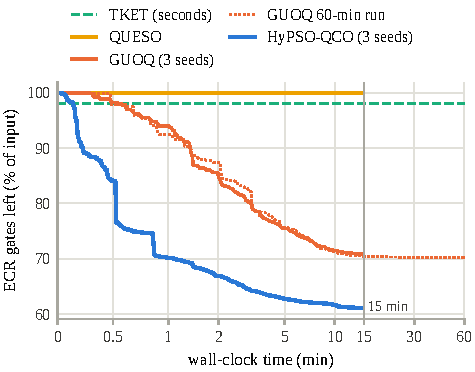
\includegraphics{rev_fig_anytime.pdf}
\caption{ECR gates left over wall-clock time, mean over the seven smaller circuits (\hypso{} and GUOQ: mean of
three seeds; dotted: GUOQ's 60-minute run; BQSKit deletion: one run). TKET runs in seconds.}
\label{fig:anytime}
\end{figure}

\textbf{\hypso{} passed GUOQ's final 60-minute result after a median of 1.2 minutes} (Fig.~\ref{fig:anytime}).
Its resynthesis removed most of its reduction in the first minutes and passed GUOQ's 60-minute result after
0.4--4.0 minutes on every one of the 21 runs, while GUOQ improved slowly and had nearly converged after
15 minutes (20.8\% at 15 and 21.5\% at 60 minutes); BQSKit stalled after its first sweeps.

\subsection{RQ4: Where the Improvement Comes From}\label{sec:rq4}
\textbf{Memetic resynthesis produced most of the ECR reduction.} In the full configuration, the swarm removed
0--10.2\% of the ECR gates on the seven smaller circuits and phase~2a 10.3--80.9\%. \textbf{At a 15-minute
budget, the swarm did not pay for itself on mapped circuits}, which is why resynthesis only is the
configuration for them: the full configuration, with a swarm phase for 25\% of the budget, lost to it on
eight of ten circuits (mean ECR margin 3.8\%, $p = 0.005$); the swarm lowers the starting point
(\cir{mult\_8}: 311 to 280), but resynthesis alone passes that point within a minute.

\textbf{Z-slot sparsification.} Without it (one seed, seven smaller circuits), the ECR count changed by
$-1.9$\% to $+4.7$\%, but the outputs had 13.5--58.7\% more physical single-qubit gates (sparsification
removed 23.6\% of them on average, and 23.2\% of all gates).

\subsection{RQ5: The Swarm as a Search Strategy}
\textbf{On logical circuits, the swarm significantly outperformed canonical PSO and the greedy compiler that
it wraps}: it reduced the primary metric by 35.0\%, 21.9\% and 6.8\% on the Clifford+T, continuous and IBM
Tokyo suites, against 33.3\%, 18.3\% and $-21.3$\% for canonical PSO (W/T/L 11/7/0, 8/3/0 and 8/0/0;
$p \le 0.004$) and 22.9\%, 13.3\% and $-0.2$\% for greedy compilation, and it was never significantly worse
than GA or SA (better than GA on two suites, $p = 0.008$ and 0.047). \textbf{Searching decomposition variants
was the largest single effect}: on six Toffoli-heavy circuits, removing the variant genes lowered the mean
gate reduction from 41.6\% to 26.1\% (6/0/0, $p = 0.016$), and a continuous relaxation of Eqs.~(3)--(4) to
40.5\% (6/0/0, $p = 0.016$); the local search, schedule genes, elitist seed, topology switch and PSO variant
made no significant difference ($p \ge 0.16$). The swarm's value thus lies in its exact decision space and
variant library, not in the particular metaheuristic.

\subsection{RQ6: Correctness}
\textbf{Every checked \hypso{} output was numerically exact}: the 30 checked outputs deviated by at most
$7.8\times10^{-8}$, and \cir{heisenberg\_32} (MPS miter) by $2.7\times10^{-10}$. TKET, QUESO, BQSKit with its
tightened threshold (at most $2.5\times10^{-7}$) and IBM's AI passes (at most $2.3\times10^{-9}$) were
numerically exact too, whereas GUOQ's outputs were approximate on \cir{heisenberg\_8} (two seeds),
\cir{hhl\_8} (one seed) and, after TKET, \cir{grover\_10} (up to $1.2\times10^{-5}$); we kept them, which can
only favour GUOQ. No tool's \cir{hubbard\_18} output could be checked end to end (the MPS miter stopped after
90 minutes at 44\% of the gates, bond dimension at least 256); \hypso{}'s is covered by its run-time checks
and by Proposition~\ref{prop:sound}(c), which bounds its deviation by $1.3\times10^{-8}$ (831 fitted and 465
TKET blocks). Two defects that verification exposed during development (\tool{SynthesiseTket} dropping small
rotations, an unchecked chunk-wise TKET pass) were fixed before the final runs.

\section{Discussion and Limitations}
\textbf{Why it wins on mapped circuits.} Mapping-preserving rewriters removed few ECR gates from Qiskit O3's
output and block resynthesis many: a level-3 transpilation leaves little redundancy that local rules reach,
but much inside blocks of three to five qubits. Deleting CNOTs only from a block's own skeleton wastes no fit
on circuits that would need re-routing, and the exact start, warm starts and Schmidt-rank pruning keep
deletion trials cheap: with the same budget and cores, BQSKit's deletion by re-instantiation removed 8.9\% of
the ECR gates, \hypso{} 33.4\%.

\textbf{Threats to validity.} The large circuits have one seed per tool, and the margins on \cir{qae\_17} and
\cir{qft\_16} (about 3\%) are small, although \hypso{}'s worst seed beat GUOQ's best run there too. GUOQ was
patched to respect the mapping, QUESO used its authors' total-gate objective, and GUOQ ran two jobs at a time
while \hypso{} ran alone (the 1-worker run addresses the compute difference). BQSKit needed a tighter threshold
than its default to return equivalent circuits, and its preprocessing can only favour it, as keeping GUOQ's
approximate outputs can only favour GUOQ. All benchmarks come from one device family and one transpiler,
success probabilities are model estimates, and equivalence is established numerically, not symbolically.

\section{Conclusion}
\hypso{} re-optimises circuits that a production transpiler has already mapped without leaving their qubits,
couplings or gate directions, combining an exact search over compiler decisions with CNOT deletion inside each
block's own skeleton under an end-to-end error bound. On ten Qiskit-O3 circuits for IBM Eagle with up to
357,535 gates, it used the fewest ECR gates of all evaluated tools on every circuit, over three seeds and
against GUOQ with four times its budget, with numerically exact outputs. Other devices and runs on hardware are
the next steps. Code, circuits, outputs and logs are available at
\url{https://anonymous.4open.science/r/hypso-qco-dac27}.

\begin{thebibliography}{38}
\footnotesize
\bibitem{mckay2017} D.~C. McKay, C.~J. Wood, S.~Sheldon, J.~M. Chow, and J.~M. Gambetta, ``Efficient Z gates
for quantum computing,'' \emph{Phys. Rev. A}, vol.~96, no.~2, p.~022330, 2017.
\bibitem{qiskit} A.~Javadi-Abhari \emph{et al.}, ``Quantum computing with Qiskit,'' arXiv:2405.08810, 2024.
\bibitem{queso} A.~Xu, A.~Molavi, L.~Pick, S.~Tannu, and A.~Albarghouthi, ``Synthesizing quantum-circuit
optimizers,'' \emph{Proc. ACM Program. Lang.}, vol.~7, no.~PLDI, pp. 140:1--140:25, 2023.
\bibitem{tket} S.~Sivarajah, S.~Dilkes, A.~Cowtan, W.~Simmons, A.~Edgington, and R.~Duncan, ``t$|$ket$\rangle$:
A retargetable compiler for NISQ devices,'' \emph{Quantum Sci. Technol.}, vol.~6, no.~1, p.~014003, 2021.
\bibitem{duncan2020} R.~Duncan, A.~Kissinger, S.~Perdrix, and J.~van~de Wetering, ``Graph-theoretic
simplification of quantum circuits with the ZX-calculus,'' \emph{Quantum}, vol.~4, p.~279, 2020.
\bibitem{pyzx} A.~Kissinger and J.~van~de Wetering, ``PyZX: Large scale automated diagrammatic reasoning,'' in
\emph{Proc. QPL}, ser. EPTCS, vol.~318, 2020, pp. 229--241.
\bibitem{voqc} K.~Hietala, R.~Rand, S.-H. Hung, X.~Wu, and M.~Hicks, ``A verified optimizer for quantum
circuits,'' \emph{Proc. ACM Program. Lang.}, vol.~5, no.~POPL, pp. 37:1--37:29, 2021.
\bibitem{qsearch} M.~G. Davis, E.~Smith, A.~Tudor, K.~Sen, I.~Siddiqi, and C.~Iancu, ``Towards optimal
topology aware quantum circuit synthesis,'' in \emph{Proc. IEEE QCE}, 2020, pp. 223--234.
\bibitem{qfast} E.~Younis, K.~Sen, K.~Yelick, and C.~Iancu, ``QFAST: Conflating search and numerical
optimization for scalable quantum circuit synthesis,'' in \emph{Proc. IEEE QCE}, 2021, pp. 232--243.
\bibitem{leap} E.~Smith \emph{et al.}, ``LEAP: Scaling numerical optimization based synthesis using an
incremental approach,'' \emph{ACM Trans. Quantum Comput.}, vol.~4, no.~1, pp. 5:1--5:23, 2023.
\bibitem{bqskit} E.~Younis, C.~C. Iancu, W.~Lavrijsen, M.~Davis, and E.~Smith, ``Berkeley quantum synthesis
toolkit (BQSKit) v1,'' Lawrence Berkeley National Laboratory, software, 2021.
\bibitem{guoq} A.~Xu, A.~Molavi, S.~Tannu, and A.~Albarghouthi, ``Optimizing quantum circuits, fast and
slow,'' in \emph{Proc. ASPLOS}, 2025.
\bibitem{nielsen} M.~A. Nielsen and I.~L. Chuang, \emph{Quantum Computation and Quantum Information}, 10th~ed.
Cambridge Univ. Press, 2010.
\bibitem{shende2004} V.~V. Shende, I.~L. Markov, and S.~S. Bullock, ``Minimal universal two-qubit
controlled-NOT-based circuits,'' \emph{Phys. Rev. A}, vol.~69, no.~6, p.~062321, 2004.
\bibitem{nam2018} Y.~Nam, N.~J. Ross, Y.~Su, A.~M. Childs, and D.~Maslov, ``Automated optimization of large
quantum circuits with continuous parameters,'' \emph{npj Quantum Inf.}, vol.~4, p.~23, 2018.
\bibitem{iten2022} R.~Iten, R.~Moyard, T.~Metger, D.~Sutter, and S.~Woerner, ``Exact and practical pattern
matching for quantum circuit optimization,'' \emph{ACM Trans. Quantum Comput.}, vol.~3, no.~1, pp.
4:1--4:41, 2022.
\bibitem{sabre} G.~Li, Y.~Ding, and Y.~Xie, ``Tackling the qubit mapping problem for NISQ-era quantum
devices,'' in \emph{Proc. ASPLOS}, 2019, pp. 1001--1014.
\bibitem{quartz} M.~Xu \emph{et al.}, ``Quartz: Superoptimization of quantum circuits,'' in \emph{Proc.
PLDI}, 2022, pp. 625--640.
\bibitem{quarl} Z.~Li \emph{et al.}, ``Quarl: A learning-based quantum circuit optimizer,'' \emph{Proc. ACM
Program. Lang.}, vol.~8, no.~OOPSLA1, pp. 114:1--114:28, 2024.
\bibitem{qfactor} A.~Kukliansky, E.~Younis, L.~Cincio, and C.~Iancu, ``QFactor: A domain-specific optimizer
for quantum circuit instantiation,'' arXiv:2306.08152, 2023.
\bibitem{kremer2024} D.~Kremer \emph{et al.}, ``Practical and efficient quantum circuit synthesis and
transpiling with reinforcement learning,'' arXiv:2405.13196, 2024.
\bibitem{dubal2025} A.~Dubal \emph{et al.}, ``Pauli network circuit synthesis with reinforcement
learning,'' arXiv:2503.14448, 2025.
\bibitem{cooper1999} K.~D. Cooper, P.~J. Schielke, and D.~Subramanian, ``Optimizing for reduced code space
using genetic algorithms,'' in \emph{Proc. LCTES}, 1999, pp. 1--9.
\bibitem{opentuner} J.~Ansel \emph{et al.}, ``OpenTuner: An extensible framework for program autotuning,''
in \emph{Proc. PACT}, 2014, pp. 303--316.
\bibitem{quetschlich2023} N.~Quetschlich, L.~Burgholzer, and R.~Wille, ``Compiler optimization for quantum
computing using reinforcement learning,'' in \emph{Proc. DAC}, 2023.
\bibitem{datta2013} K.~Datta, I.~Sengupta, and H.~Rahaman, ``Particle swarm optimization based reversible
circuit synthesis using mixed control Toffoli gates,'' \emph{J. Low Power Electron.}, 2013.
\bibitem{zelinka2023} I.~Zelinka, L.~Kojeck\'y, and M.~Lampart, ``iSOMA swarm intelligence algorithm in
synthesis of quantum computing circuits,'' \emph{Appl. Soft Comput.}, 2023.
\bibitem{hidayat2025} M.~H.~N. Hidayat and T.~C. Cheah, ``Particle swarm optimization for quantum circuit
synthesis: Performance analysis and insights,'' arXiv:2507.02898, 2025.
\bibitem{strasser2016} S.~Strasser, R.~Goodman, J.~Sheppard, and S.~Butcher, ``A new discrete particle swarm
optimization algorithm,'' in \emph{Proc. GECCO}, 2016, pp. 53--60.
\bibitem{kennedy1995} J.~Kennedy and R.~Eberhart, ``Particle swarm optimization,'' in \emph{Proc. ICNN},
vol.~4, 1995, pp. 1942--1948.
\bibitem{clerc2002} M.~Clerc and J.~Kennedy, ``The particle swarm---explosion, stability, and convergence in
a multidimensional complex space,'' \emph{IEEE Trans. Evol. Comput.}, vol.~6, no.~1, pp. 58--73, 2002.
\bibitem{sun2004} J.~Sun, B.~Feng, and W.~Xu, ``Particle swarm optimization with particles having quantum
behavior,'' in \emph{Proc. IEEE CEC}, 2004, pp. 325--331.
\bibitem{kennedy2002} J.~Kennedy and R.~Mendes, ``Population structure and particle swarm performance,'' in
\emph{Proc. IEEE CEC}, 2002, pp. 1671--1676.
\bibitem{tizhoosh2005} H.~R. Tizhoosh, ``Opposition-based learning: A new scheme for machine intelligence,''
in \emph{Proc. CIMCA}, 2005, pp. 695--701.
\bibitem{thierens2005} D.~Thierens, ``An adaptive pursuit strategy for allocating operator probabilities,''
in \emph{Proc. GECCO}, 2005, pp. 1539--1546.
\bibitem{nocedal} J.~Nocedal and S.~J. Wright, \emph{Numerical Optimization}, 2nd~ed. Springer, 2006.
\bibitem{conover} W.~J. Conover, \emph{Practical Nonparametric Statistics}, 3rd~ed. Wiley, 1999.
\bibitem{eiben} A.~E. Eiben and J.~E. Smith, \emph{Introduction to Evolutionary Computing}, 2nd~ed.
Springer, 2015.
\end{thebibliography}

\end{document}
